\chapter{Analyses}

\label{ch:analysis}

Before designing an educational product, it is important that the designer first acquaints himself with the extrinsic factors important to this product. In order to discover the important characteristics of these factors, \citeA{instructionaldesign} enlist three types of analyses to be conducted, together with steps for conducting them. These are an analysis of the context, encompassing the needs of the users, and the environmental characteristics, an analysis of the learner, and an analysis of the learning task. Although these analyses are more targeted towards instructional design, and therefore more focused on a specific group being taught specific content, these analyses will still provide relevant information for the design choices and the evaluation. However, the steps will be adjusted and generalised or even omitted in order to fit the design of the more generic learning tool. The information gathered in order to conduct these analyses mainly stems from meetings with one of the teachers. This might not be the most reliable source of information because of the lack of triangulation, and should therefore not be taken as insight in the curriculum of Dutch Literature courses in secondary education, but rather as context information relevant to the design.

\section{Analysis of the learning context}

As already stated in the \nameref{sec:intro_evaluation} section on page~\pageref{sec:intro_evaluation}, the evaluation of the flashmap system will be evaluated within the Dutch secondary school Stedelijk Lyceum, with students having to learn about the Renaissance genres in Dutch Literature. This context will be further investigated within this section, starting with the Needs Assessment \cite{instructionaldesign}. Because although the general needs for a flashmap system are already described in the \nameref{ch:problem}, it is still important to investigate the specific needs of the context where the programm will be implemented.

\subsection{Needs assessment}

According to \citeA{instructionaldesign}, the first step in a needs assessment is to assess whether there is a problem, and what the nature is of the problem (see figure~\ref{fig:needsassessment}, mostly to identify the problem, but also in order to assess whether the innovation model or the discrepancy model applies for determining the needs. The first step is to assess whether there really is a problem in order to establish the general need. During the meetings, the teacher did confirm the need for better retention and comprehension of the content, and indicated that most of the time the students only learned the night before the exam in order to get a high (enough) grade and consequently forget everything again. This is not only wasteful of the effort of learning, but also causes problems when the knowledge becomes relevant again in the next chapter. The cause of this problem therefore definitely lies within the learning process, and could possibly be improved by the use of a flashcard or flashmap system, so it can be concluded that there is indeed a problem caused by learning, and it is thereby useful to proceed with the next phase of the assessment. Finally, \citeA{instructionaldesign} finally state that if there already exists instruction for the relevant learning goals, since if so than one has to proceed by using the discrepancy model, and otherwise by using the innovation model. The new tool is only there to enhance the current learning process by adding an additional activity, rather than adding new learning goals to an empty space in the curriculum. Thereby, from an instructional perspecticve, the flashcard or flashmap system is only an improvement of the currently existing instructional activities rather than a new innovation, and therefore the discrepancy model will be used.

\begin{figure}
    \centering
    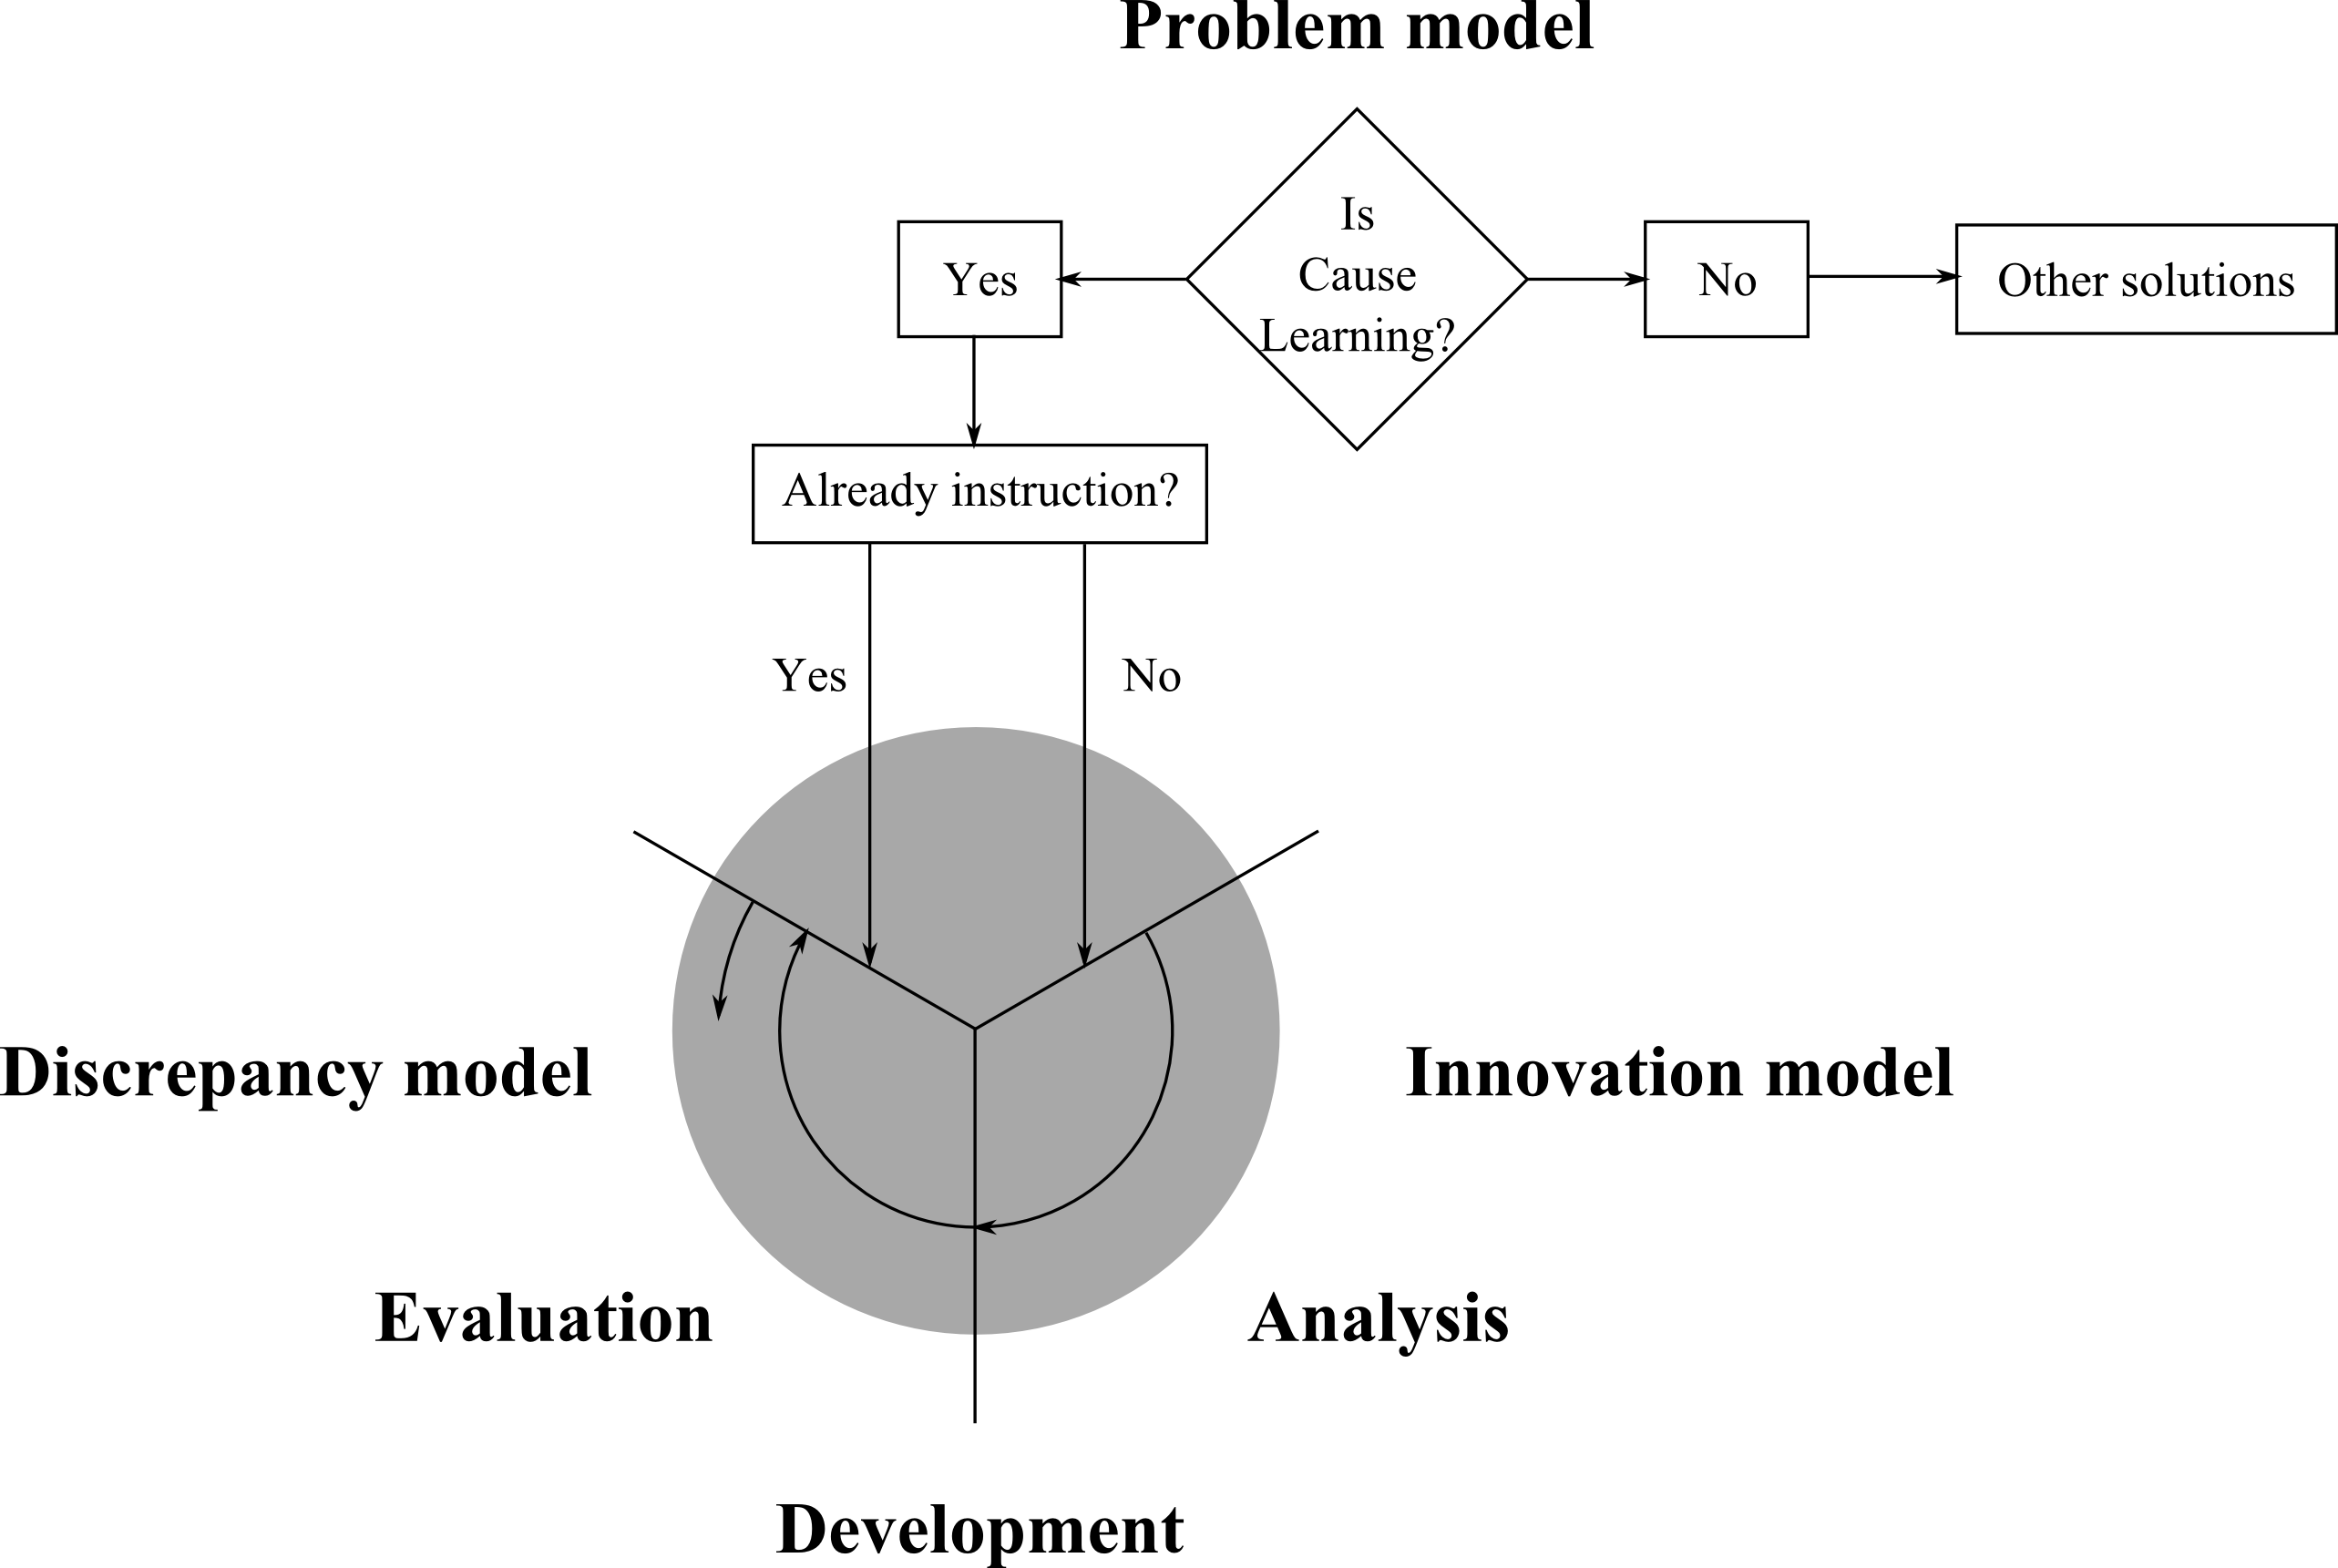
\includegraphics[width=\textwidth]{img/needsassessment.png}
    \caption{The three sides of needs assessment \protect\cite{instructionaldesign}}
    \label{fig:needsassessment}
\end{figure}

As can be seen in figure~\ref{fig:needsassessment}, the discrepancy model for needs assessment uses evaluative methods rather than analytical in order to establish the needs within the organisation. These methods include establishing the goals of the instructional system, determining how well these goals are currently being achieved, determining the gaps, prioritising the gaps, and determining which gaps are instructional needs (or in this case, educational needs). These remaining gaps can consecutively be used as a basis for determining the general use cases of the educational product. Normally an instructional designer tries to come into the organisation as a tabula rasa, without any preconceptions on what he would want to achieve and merely try to solve the real problem apparent in the organisation itself. However, because this design is theory driven rather than problem driven, it was merely checked with the teacher whether the problems stated in literature are also a problem here.

The first step was to confirm whether the goal stated by \citeA{glaserfield} of wanting students to memorise many facts in a meaningful way. Upon prompting the teacher what she deemed to be most important for her students to take away from her lessons was for them to become more familiar with the Dutch Renaissance writers or work. For example, she stated that she wanted the students to at least recognise important names when they saw a street name such as the "P.C. Hooftstraat" or the "Vondelpark". She also would like the students to be able to distinguish between different genres of literature, such as the \emph{sonnet} or \emph{emblematiek}. Based on these statements, the goals within the context are in line with students memorising and understanding all of the facts, without them being too ambitious. There are also differences between her and the other two teachers, they namely only offered the materials presented within the books, whereas she offered some additional content which the students also needed to master. However, she also stated that she would be responsible for the extra materials, and that the tool could be only to learn the textbook materials. Finally, she provided a test from the previous year to offer some more concrete examples of what she wanted the students to know, of which an English translation is included in the appendix on page~\pageref{ch:exampletest}. From this test, more goals can be extrapolated, such as students having to not only distinguish different genres, but also to define them or provide characteristics, and recognise the application of these features in both examples of the time periods as well as modern examples. Furthermore, they have to be able to relate the famous writers and writings to the genres.

According to the teacher, the students were mostly able to score points on the reproduction questions, such as having them to provide definitions or enlisting characteristics of genres. Thereby, most students were able to (barely) pass the test, which was already regarded as an important achievement, however minimal it might be. In this regard, the teachers already had scaled down their expectations of the students quite a bit to a realistic and feasible bar. The teacher also tried to make the material more appealing by focusing on examples, with succes.

However, as already indicated before, the main problem of students learning just before the exam and then forgetting about it remained an issue for the teacher, and more improvements could be made towards creating an understanding of the content by the students. Furthermore, although the examples make the content more appealing, according to the teacher students generally still did not experience the topic of Dutch renaissance literature as engaging or interesting (see also \citeNP{heemskerk}). Finally, most of the students would rapidly forget what they have learned after the exam, which the teacher did experience as wasteful. Therefore, the general categories of improvement can be enlisted as the students insufficiently understanding the content, not being immersed or engaged with the content (adequately), and retaining the acquired knowledge for a too short period of time.

Within the context of the Flashmap system, for now only the insufficient comprehension and retention of the content are prioritised, since there is no real evidence within the studied literature that the tool would also make content more immersive (although this could still be a side effect of the tool). These gaps are both instructional needs and are therefore appropriate gaps to tackle within the design.

\subsection{The learning environment}

\subsubsection{The school}

The Stedelijk Lyceum is one of the two major schools in Enschede (together with the Bonhoeffer College), which has an open denomination and provides education to 3339 students. It consists of 7 minor schools on different locations, of which the Kottenpark location is approached within this project. The location was approved by the Dutch Inspection of Education \cite{inspectierapport} based on analysing relevant documents, visiting the school and observing lessons, conduct interviews with relevant agents (such as teachers and students), and discussing the results with the director and administrator. They reported that the school climate is very positive and safe, and that the teachers have enough professional space to develop themselves. However, they also found that the exam results are some years around the national average, and some years below. The possible reasons they provided were that teachers usually focus on what students have to do instead of what they have to learn, and that they apply differentiation to a lesser extend. Yet, the school now makes use of student monitoring systems, so that they can better tackle problems like language deficiencies and the like.

\subsubsection{The curricular spiderweb}

Although \citeA{instructionaldesign} do enlist some of the steps necessary for describing the learning environment, \citeA{curricularspiderweb} provides a more widely used and thorough model, and therefore this will be used instead. This model is depicted in figure~\ref{fig:spiderweb}, and displays the relevant components which have to be taken into account for implementation of educational innovations. They are arranged as a spider's web, nog only illustrating their many inter-connections, but also underlining the vulnerability of the whole implementation. These aspects will be visited one by one from the perspective on the school, since the learner will be addressed separately in the next section.

\begin{figure}
    \centering
    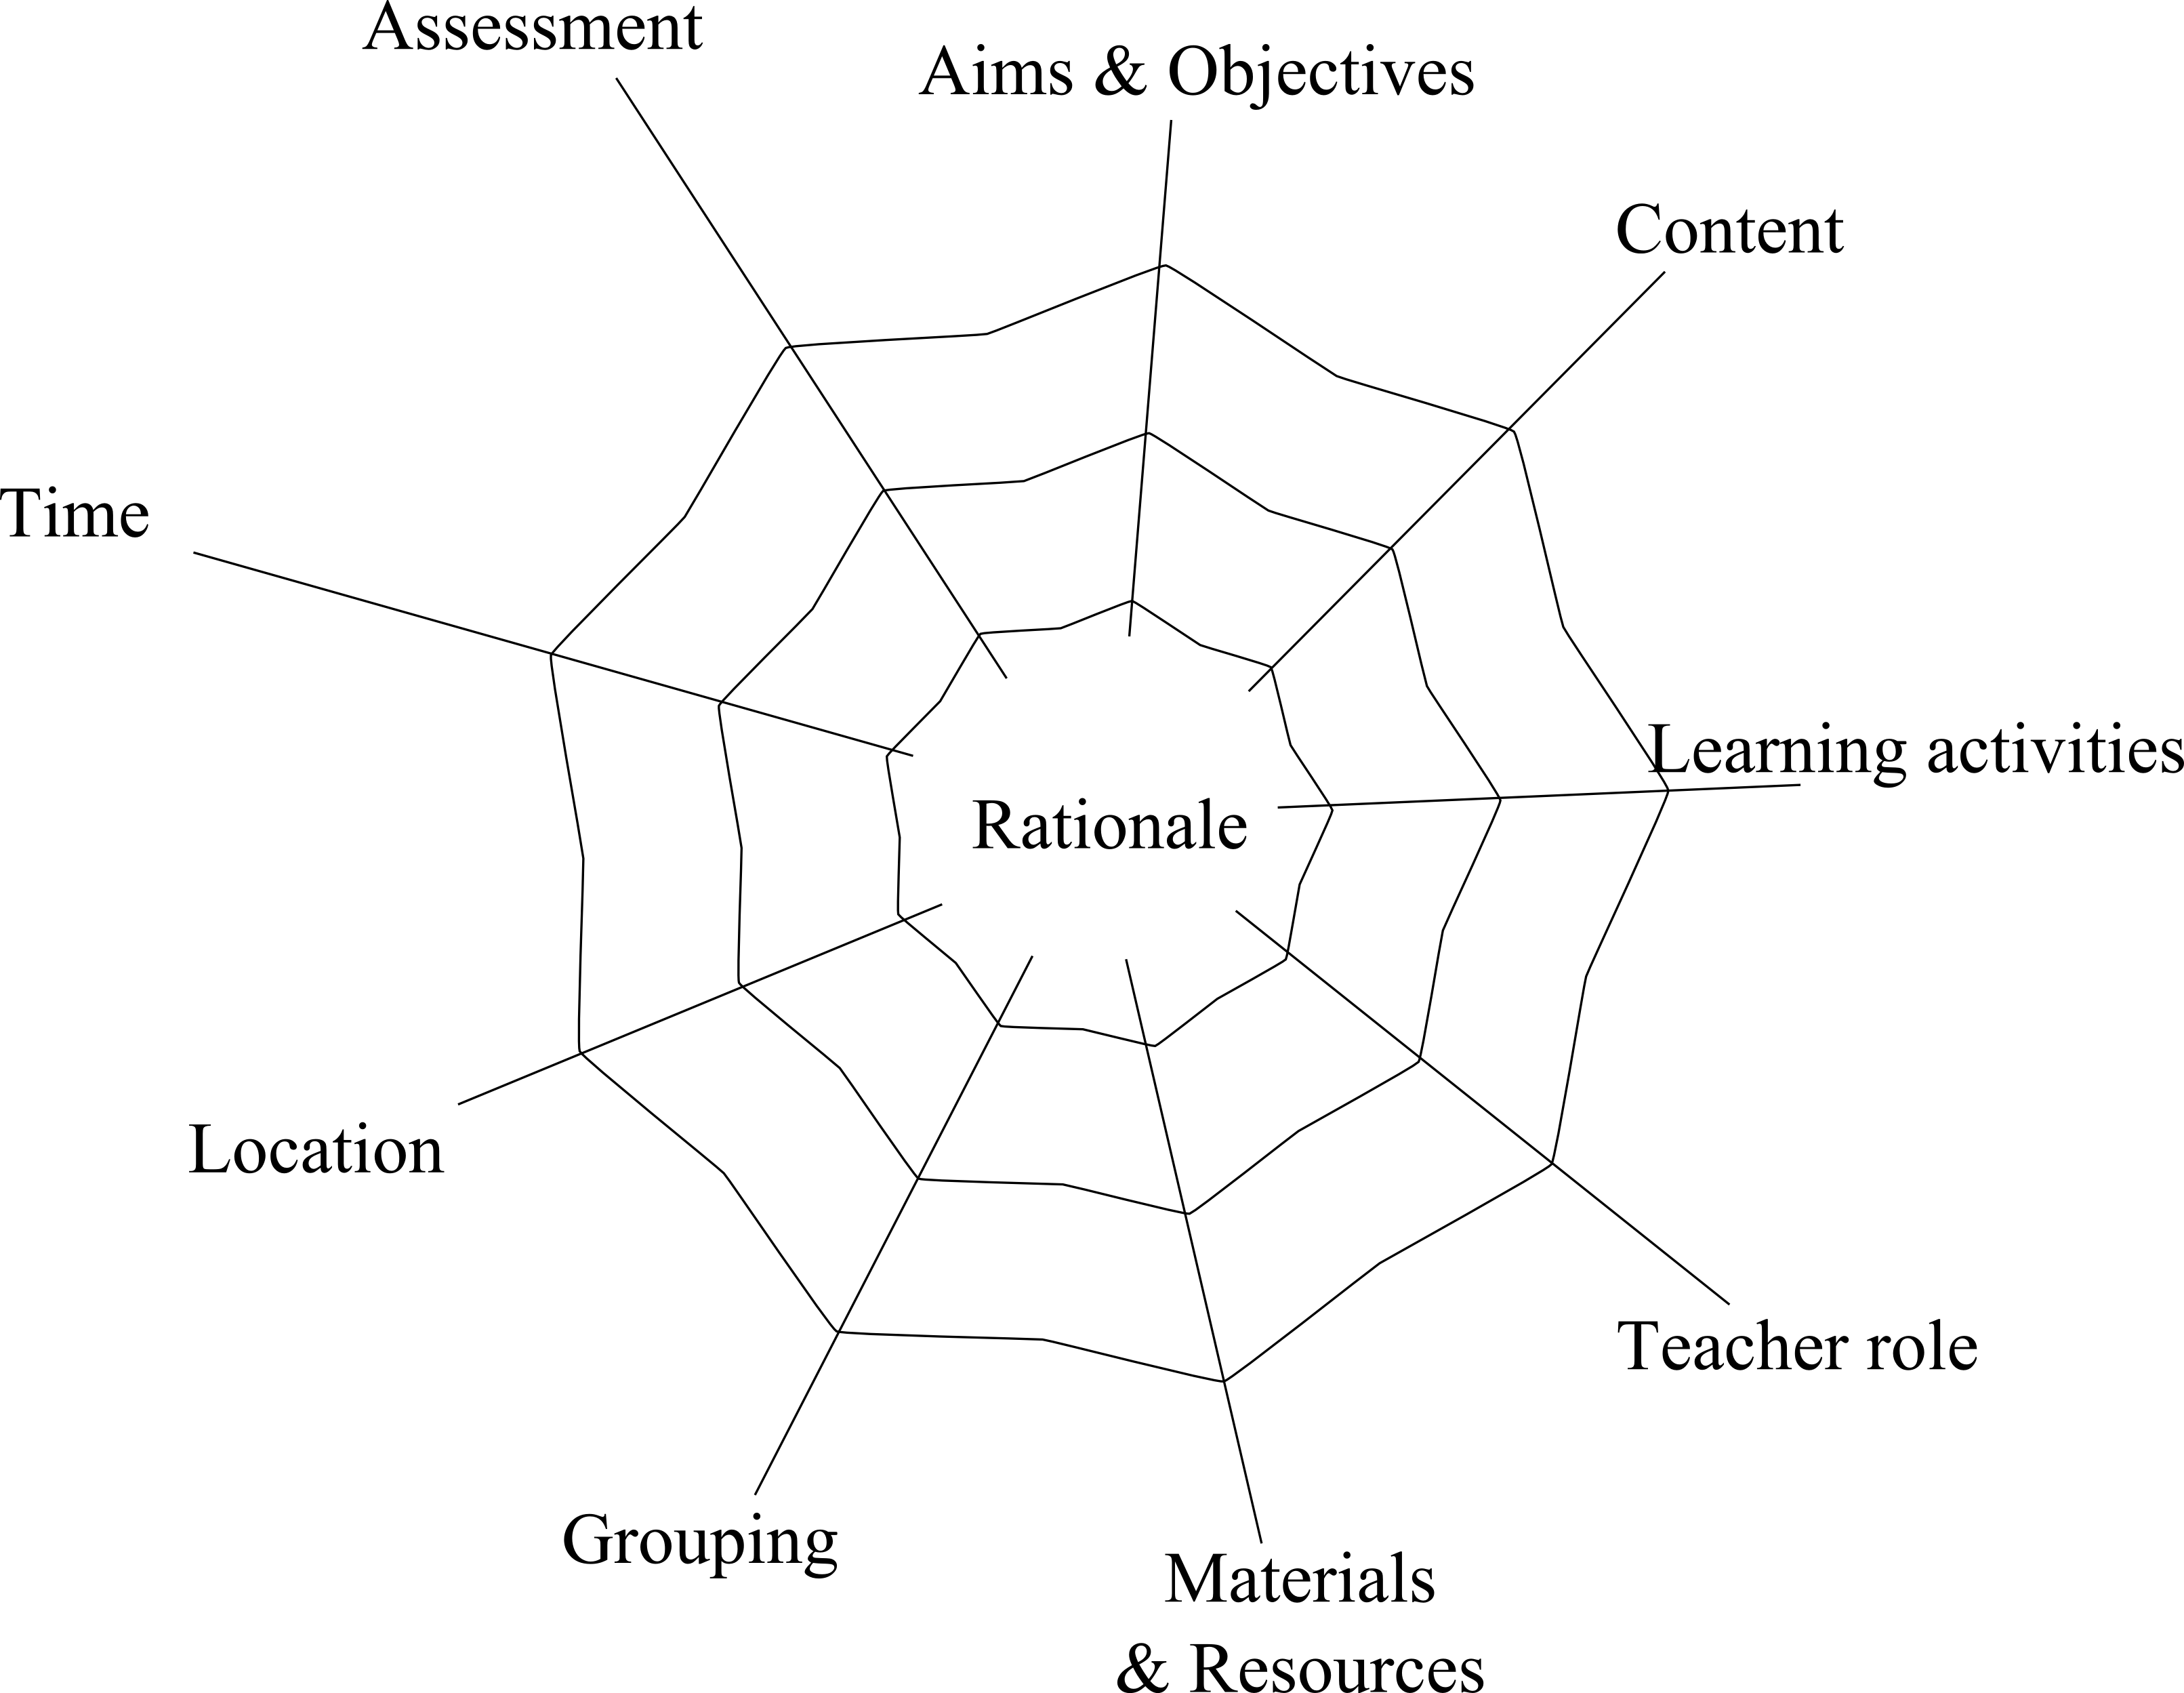
\includegraphics[width=0.7\textwidth]{img/curricular_spiderweb.png}
    \caption{The curricular spiderweb \protect\cite{curricularspiderweb}}
    \label{fig:spiderweb}
\end{figure}

The central aspect, \emph{rationale} (or vision), represents the question why students are learning the content in the first place. From the previously visited educational philosophies, one could make many arguments why students should familiarise themselves with Dutch renaissance literature: from a perennialistic or essentialistic perspective one could argue that it is the only way this knowledge can be transferred to the next generation and keeping it relevant; a progressivist could argue that one should first be familiar with older genres before one improve upon them or create new genres; reconstructivists might deem it important since it explains something about the national heritage, and thereby point out the flaws of the old ways; and finally an existentialist sees art in general as a meaningful way for self discovery. This intrinsic motivation is heavily dependent on the individual motivations and philosophy of the teacher. Most of these arguments are represented in diverse Dutch opinion pieces (e.g. \citeNP{opinion1, opinion2}). In the case of the consulted teacher, the arguments provided seemed to come mainly from the perennialistic and essentialistic perspective, namely that the content is part of our cultural identity and thereby important \emph{an sich}. However, she also indicated the existentialist self-discovery to be valuable. Furthermore, schools are extrinsically motivated to teach the material, since it has to demonstrate to society (mainly the exam committee) that their students have mastered this content. This is mainly related to subdomain E2 and E3 in the Dutch national exam programm, which states that a student can recognise and distinct between literary textgenres, and apply literary concepts in the interpretation of literary work; and that a student can provide the outlines of the (Dutch) literature history, and place literary works in this historical perspective.

Both the content and aims \& goals are already stated in the needs assessment, and can be summarised as: Students have to learn about prominent writers and genres within the context of Dutch renaissance literature; and have to be able to recognise important names and concepts, be able to define them or relate them to each other, and apply features of genres in examples of texts.

The course consists of two different types of learning activities, which are classroom instruction, and individual learning at home by the students. Their are two sessions of classroom instruction, both lasting 50 minutes, in which the 100 students are divided over the three teachers in static groups on separate locations. These lessons take place over the course of two weeks, with one lesson provided in one week. Within these lessons, the teachers transfer knowledge and provide excersises for the students. Outside of the lessons, the students still have to study the textbook Laagland individually \cite{laagland}, which contains all of the materials which will be prompted on a final written assessment. As already stated before, the teacher indicated this activity mostly to take place on the evening before the assessment, and only on a superficial level. Finally, this assessment takes place in the second week after the final instruction, and will be similar to the example test included in the appendix on page~\ref{ch:exampletest}.

The teacher stated that the course mainly consisted of the rote memorisation of facts, and that she was still doubtful whether the students would actually be willing to participate in the evaluation of the Flashmap system. Yet, she did see the general use of the tool for achieving the learning goals, and therefore still seemed to be enthusiastic in cooperation and encouraging the students to participate. The only two technical problems are that there is not too much time for extra activities within the lesson plan and the teachers being quite busy themselves, and that the technological possibilities within the classroom are limited. Within the classroom, only a couple of computers are available for use, and still run relatively old software. Therefore, the activities envolved in using the flashmap have to target the individual learning of students, since they have more time outside of the lesson plan, and mostly do possess the hardware and software necessary to run the software.

\section{Analysis of the learner}

%TODO: introduction of this analysis

\subsection{Four categories of learner characteristics}

\citeA{instructionaldesign} propose a methodology for assessing a learner which focuses on two axes: Stable and Changing, and Similarities and Differences, creating 4 categories. Within these categories, different types of learner characteristics, which are enlisted in table~\ref{tab:catslearner}. Stable similarities involve characteristics which are similar among people and do not change over time, such as sensory capabilities and their corresponding perceptual responses, the way people process information, and finally the ways and conditions in which people learn. Stable differences relate to characteristics different among people but stable over time, such as certain aptitudes, cognitive styles, psychosocial traits, or inheritary traits such as gender, ethnicity \& racial group. Changing similarities are similarities that do change over time, these characteristics are mainly attributed towards development processes. Finally, changing differences are differences in development accross people, which can mainly be attributed towards different upbringings or interests. Instead of visiting the learner characteristic according to each above mentioned category, \citeA{instructionaldesign} propose an more conveniently arranged outline which will be used in the next sections, albeit slightly altered in order to fit the current project.

\begin{table}[ht]
\centering
\begin{tabular}{l|l|l|}
         & Similarities                                                                                                                      & Differences                                                                                                                        \\ \hline
Stable   & \begin{tabular}[c]{@{}l@{}}Sensory Capacities\\ Information processing\\ Types and conditions of learning\end{tabular}            & \begin{tabular}[c]{@{}l@{}}Aptitudes\\ Cognitive Styles\\ Psychosocial traits\\ Gender, Ethnicity, \& Racial Group\end{tabular}    \\ \hline
Changing & \begin{tabular}[c]{@{}l@{}}Development Processes:\\ - Intellectual\\ - Language\\ - Psychosocial\\ - Moral\\ - Other\end{tabular} & \begin{tabular}[c]{@{}l@{}}Developmental state:\\ - Intellectual\\ - Other\\ Prior learning:\\ - General\\ - Specific\end{tabular} \\ \hline
\end{tabular}
\caption{The four categories of learner characteristics \protect\cite{instructionaldesign}}
\label{tab:catslearner}
\end{table}

\subsection{Physiological characteristics}

\label{subsec:physiologicalchar}

The students who will participate in the research are enrolled in grade 4 of Dutch secondary education, and therefore should be around the age of 16-17, with some deviations due to students either having skipped or repeated a grade. Therefore, the students are generally considered to be either at the end of puberty, or the beginning of young adolescence. Chapter \refname{ch:theory} on page~\pageref{ch:theory} already provides general theories about the learning process within the brain. However, during late puberty and early adolesence, the brain is still heavily in development, especially the prefrontal cortex. \cite{blakemore}. These changes might be even more relevant than the pure chronological age, and therefore they will have to be elaborated on further before delving into the cognitive characteristics.

\begin{figure}
    \centering
    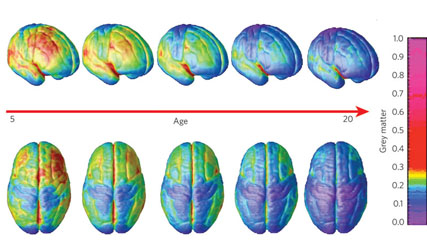
\includegraphics[width=.7\textwidth]{img/braindevelopment.png}
    \caption{The MRI scans from the longitudinal study conducted by \protect\citeA{giedd}, showing the maturation of the brain during childhood and adolescence}
    \label{fig:braindevelopment}
\end{figure}

In order to map out the changes in the adolescent brain, \citeA{giedd} performed a longitudinal MRI study of the brain development during this period, of which the results are displayed in figure~\ref{fig:braindevelopment}. Within this study, three themes emerged within the adolescent development of the brain:

\begin{enumerate}
    \item After a peak in growth of both braincells, connections and neurotransmitters during childhood, one can see a decline in adolescence;
    \item The connectivity between different regions of the brain increases;
    \item A new balance is formed among frontal and limbic lobes.
\end{enumerate}

The first theme is a result for the brain becoming more streamlined after having collected a lot of information during late childhood, making it more efficient (see also page~\pageref{subsec:interferencedecay} on \nameref{subsec:interferencedecay}). This is also known as peak plasticity, which after that again decreases over time. \citeA{powell} describes this phenomenon as \emph{Use it or lose it}, since the brain rigorously selects the specific memories which are activated during this time. The second theme refers to the strengthening of specific memories, which are enhanced during that period. Finally, during adolescence a shift is made from "cold" to "hot" cognition, where the former relates to hypothetical, low-emotion reactions, and the latter to high arousal decision making, strongly influenced by peer pressure and real, direct consequences. This is strongly related to the prefrontal cortex being strongly developed, resulting in the teenage brain to rely stronger on the amygdala: the more emotional, impulsive area of the brain.

The developmental level of the prefrontal cortex has also been found to positively correlate with the IQ of students, more so than other regions of the brain, which is an indication of this development to be the most influential for the cognitive development within adolescents.

The development of the prefrontal cortex has important consequences for the cognitive development of adolescents. They become more capable of abstract, multidimensional, planned and hypothetical thinking in comparison to children \cite{steinberg}. Adolescents also tend to use their hippocampus more often during executing certain tasks \cite{finn}, possibly due to the highly increased plasticity of the brain.

\subsection{Cognitive characteristics}

The Dutch highschool is subdivided into three main categories, which are VMBO, HAVO and VWO, ranking from lower to higher rates of academic achievement and expectations. The students targeted within this projects are VWO-students, which means that they are most likely to have a relatively high IQ, and are quite apt of learning and passing for written tests. Furthermore, at the beginning of grade 4 of VWO, students are allowed to choose between a nature profile or a society profile, determining whether they have respectively have more STEM subjects (such as math or biology), or more subjects related to language, humanities or economy. Therefore, where students who chose the nature profile are generally more apt to apply logic to technical problems, those who chose the society profile are generally more apt and used to learning information by reading texts. This makes up for different specific aptitudes within this specific Dutch literature course, where reading skills are more relevant. VWO-students are also subdivided into Gymnasium and Atheneum students, where the former group outside of the regular curriculum also has to learn classical languages (Latin and Ancient Greek) and culture. Because the Dutch renaissance literature has a lot of connections with classical genres, Gymnasium students might have an advantage in prior knowledge. Furthermore, all students should have learned about the relevant time period in their history classes prior to this course (e.g. the Spanish War, the Lutheran reformation etc.), providing with the relevant knowledge to understand the context of Dutch renaissance literature. Finally, the students have received a similar instruction on Dutch medieval literature, which is also relvant for concepts in the renaissance literature, such as the \emph{Mecenas}, the \emph{Lyriek} and \emph{Rederijkers}.

\subsection{Social characteristics}

This section covers the stage of moral development, the socioeconomic status, the racial or ethnic background, and the religious denominations of the students. The stage of moral development is relevant since it influences the individual decisions the students are likely to make. The socioeconomic status (SES) is found to influence the academic achievement of students, since they are predictors of both the safety of the home situation and the support from the parents. Furthermore, racial and ethnic backgrounds might influence the attitudes that students have towards certain topics. Finally, since the subject of Dutch renaissance literature is heavily influenced by religion, especially the reformed church, the denomination influences the perspective of the student towards the subject, and determines a certain amount of prior knowledge. The SES, the racial or ethnic background, and the religion have not been investigated within the target group, so instead public available statistics from the Dutch social and cultural plan agency (\emph{Sociaal en Cultureel Planbureau}, SCP), the Ministry of the Interior and Kingdom Relations (\emph{Ministerie van Binnenlandse Zaken en Koninkrijksrelaties}, BZK),  and Statistics Netherlands (\emph{Centraal bureau voor de Statistiek}, CBS) were used.

%Stage of moral development

%The region around Enschede has a lesser income in comparison to the national income: where the national average lies around 33.2 thousand euros, the average income in Enschede is 27.1 thousand euros per household. This is also true when looking at the median (28 vs 23.1 thousand) and for the average and median standardised incomes (23.5 vs 19.7 and 20.9 vs 17.9 thousand euros), where the latter are corrected for differences in size and composition of a household (see also table~\ref{tab:income}). 

Every four years the SCP publishes data reporting the socioeconomic status (SES) of postal areas in the Netherlands \cite{scp}. The SES is based on three variables of the people living their, namely their education, their spendable income, and their position on the labour market. The data about the postal area of the school is displayed in table~\ref{tab:scpses}, together with the data of its two major neighbouring postal areas. As one can see, all of the values are below the national average SES, and that the surrounding postal areas have a lower SES than the school's postal area. However, academic achievement and socioeconomic status are highly correlated \cite{academicsocioeconomic}, and given that the approached students are enrolled on the VWO level one might expect them to come from households with higher incomes. Furthermore, the BZK frequently publishes indications of living circumstances \cite{bzk}, which is specified with smaller areas and is found to correlate with the SES \cite{knol}. On this map, the area Bolhaar scores a 0.3 in comparison to the national average. It could therefore be that the actual SES of the students of the school is somewhat higher than indicated within the table, especially since there is also a university campus within the same postal area, where low income university students live.

\begin{table}[]
    \centering
    \begin{tabular}{|p{2cm}|p{2cm}|p{2cm}|p{2cm}|p{2cm}|}
        \hline
        Postal code & Number of residents & Number of households & SES score & SES rank \\ \hline
        National &  &  & 0.28 &  \\ \hline
        7521 & 9555 & 4624 & -1.28 & 3254 \\ \hline
        \textbf{7522} & \textbf{7100} & \textbf{4551} & \textbf{-0.37} & \textbf{2792} \\ \hline
        7523 & 12180 & 6060 & -1.62 & 3333 \\ \hline
    \end{tabular}
    \caption{Indicators of socioeconomic status on both national and postal code levels \protect\cite{scp}}
\label{tab:scpses}
\end{table}

%Racial/ethnic background, affiliations

Among other data, the CBS offers descriptives of students, categorised per national district. This descriptive data entails information about the age, sex, type of education, and ethnicity of students, and the interactions among these variables \cite{cbsethn}. From this data, descriptives about 16-17 year old students from Enschede enrolled in vwo grade 3-6 was extracted, displaying their age and ethnicities. 23.06\% of the 16-17 year old students are enrolled in VWO, where 43.97\% is male and 56.03\% is female. The distribution of ethnicity is visualised in figure~\ref{fig:ethnicitychart}. 76.56\% of the students are native and 31.09\% are non-native. 9.16\% of the students is western non-native, and 21.92\% is non-western non-native. The CBS defines a non-western non-native as an non-native originating from Afrika, Latin-Amerika and Asia (except for Indonesia and Japan) or Turkey. The most prevalent non-western ethnicity is Turkish, with 8.08\%.

\begin{figure}
    \centering
    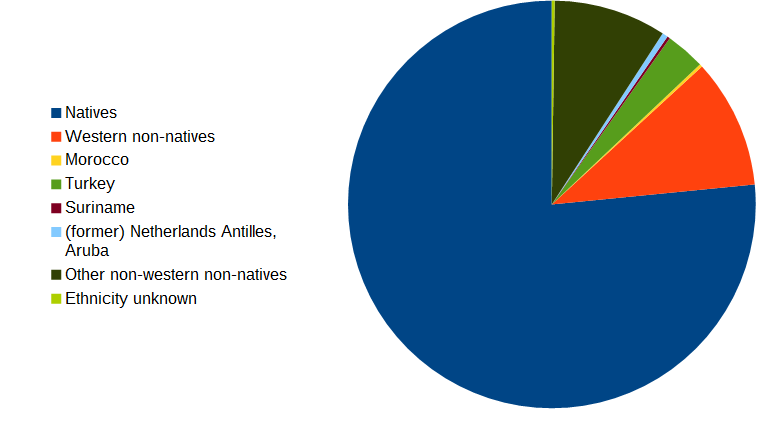
\includegraphics[width=0.7\textwidth]{img/ethnicitychart.png}
    \caption{The distribution of ethnicities among 16-17 year old vwo students of education type vwo3-6 \protect\cite{cbsethn}}
    \label{fig:ethnicitychart}
\end{figure}

Finally, the CBS also offers statistics about religious denominations \cite{cbsdenom}, which state that 57\% of the people in the province of Overijssel is affiliated to a church. These affiliations are split up in different religions: 22\% Roman-Catholic, 8\% Protestant, 12\% Dutch Reformed, 7\% Continental Reformed, 4\% Islam, and 5\% miscellaneous (see figure~\ref{fig:denominations}. 43\% is not affiliated to any church, however this does not necessarily entail that they do not have a religious worldview. Data is also offered on how frequent people visit the church: 14\% visits every week or more often, 4\% two or three times a month, 4\% once a month, 8\% less than once a month, and finally 70\% (almost) never (see figure~\ref{fig:churchvisits}. This would indicate that although there is a majority affiliated with a certain church, most of the people do not actively take part in their respective community. There are also more specific statistics available about the region of Twente only \cite{cbsdenomold}, however these are older and might already have changed significantly over the last 13 years. Yet, they state that Twente is more religious than the overal province of Overijssel. Unfortunately, there are no statistics available about Enschede only. Finally, the school of the target group has an open (i.e. non-religious) denomination, whereas the other large school in Enschede has a christian denomination, so one might expect mainly the students without any strong religious views to choose for this school.

\begin{figure}
    \centering
    \begin{subfigure}[b]{0.7\textwidth}
        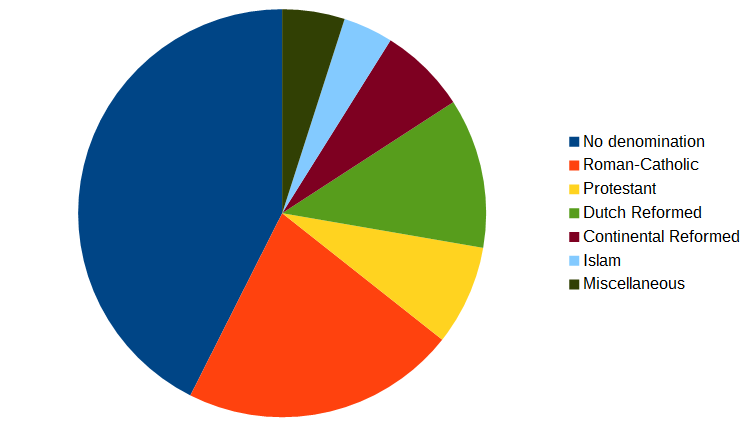
\includegraphics[width=\textwidth]{img/denominations.png}
        \begin{center}
            \caption{A distribution of church affiliations}
        \end{center}
        \label{fig:denominations}
    \end{subfigure}
    \begin{subfigure}[b]{0.7\textwidth}
        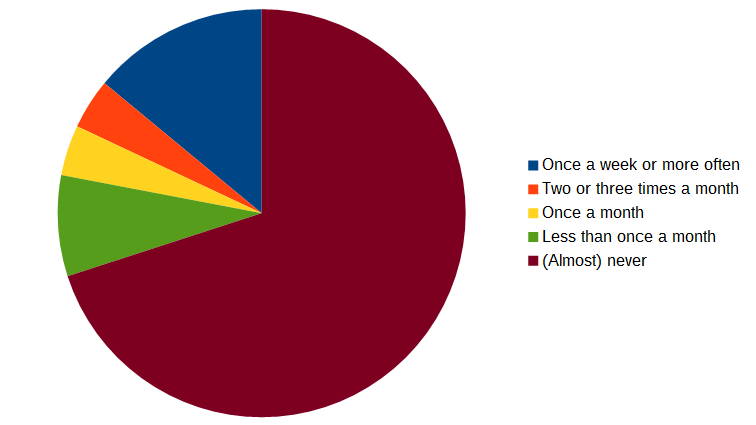
\includegraphics[width=\textwidth]{img/churchvisits.png}
        \begin{center}
            \caption{The distribution of frequencies of church visits within the group of people affiliated to a church}
        \end{center}
        \label{fig:churchvisits}
    \end{subfigure}
    \caption{Denominations within the region of Twente \protect\cite{cbsdenom}}
\end{figure}

\subsection{Affective characteristics}

The influences on the students attitudes can be mainly categorised into two factors: the natural factors and the nurtural factors, which will be described in seperate paragraphs below.

Within the section \nameref{subsec:physiologicalchar} on page~\pageref{subsec:physiologicalchar} it was already described that students rely mainly on their amygdalic systems instead of their prefrontal cortex during young adolescence. According to \citeA{steinberg}, this mainly leads to reward-seeking behaviour, peer-reliance, risk-taking, and poor decision making. This has the consequence of students being heavily influenced by the direct consequences of their actions rather than the long-term benefits or drawbacks, which are in a lot of cases related to social rewards and stimuli rather than cognitive rewards. Furthermore, they are more likely to take certain risks in order to gain these rewards, possibly causing procrastination-like behaviour until the risk of failing the exam is too large. This is also heavily related to poor decision making, at least in the long term. These types of behaviour are also in line with what the teacher stated about her students, namely that they postpone their studying behaviours until the last possible moment (in most cases the night before the exam), and that their strategies are not more elaborate than just reading or even skimming through the chapter.



%Perceptions towards history by different ethnicities
%Religious influence
%Home situation

%Perceptions toward classical art (atheneum vs gymnasium and nature vs culture profiles)

% How to relate this framework with a personal framework?
%   How is this done in the textbook

% Maybe use the outline at the end of the chapter instead for the structure

\section{Analysis of the task}

% Description of the different sections within the textbook, and reference to the concept mapping design chapter
